\usetikzlibrary{arrows.meta}
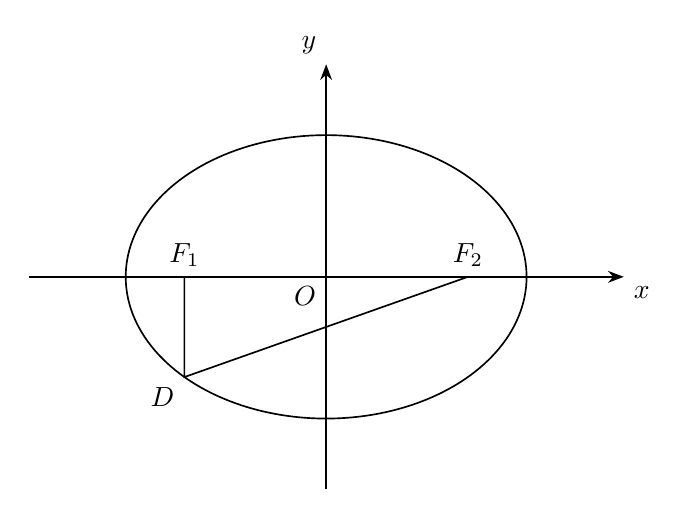
\begin{tikzpicture}[x=1.8cm,y=1.8cm,line width=.6pt,font=\normalsize,>=Stealth]
\draw[->] (-2.1,0)--(2.1,0) node[below right] {$x$};
\draw[->] (0,-1.5)--(0,1.5) node[above left] {$y$};
\draw[solid] plot[variable=\t,domain=0:360,samples=180] ({sqrt(2)*cos(\t)},{sin(\t)});
\coordinate (F1) at (-1,0);
\coordinate (F2) at (1,0);
\coordinate (O) at (0,0);
\coordinate (D) at (-1,-0.70710678);
\draw[solid] (F1)--(D)--(F2);
\node[above] at (F1) {$F_{1}$};
\node[above] at (F2) {$F_{2}$};
\node[below left] at (O) {$O$};
\node[below left] at (D) {$D$};
\end{tikzpicture}
